\documentclass[border=10pt]{standalone}

\usepackage{tikz}
\usepackage{tikzsymbols}
\usetikzlibrary{calc,patterns,shapes.geometric}

\def\centerarc[#1](#2)(#3:#4:#5){\draw[#1] ($(#2)+({#5*cos(#3)},{#5*sin(#3)})$) arc (#3:#4:#5);}

\begin{document}
	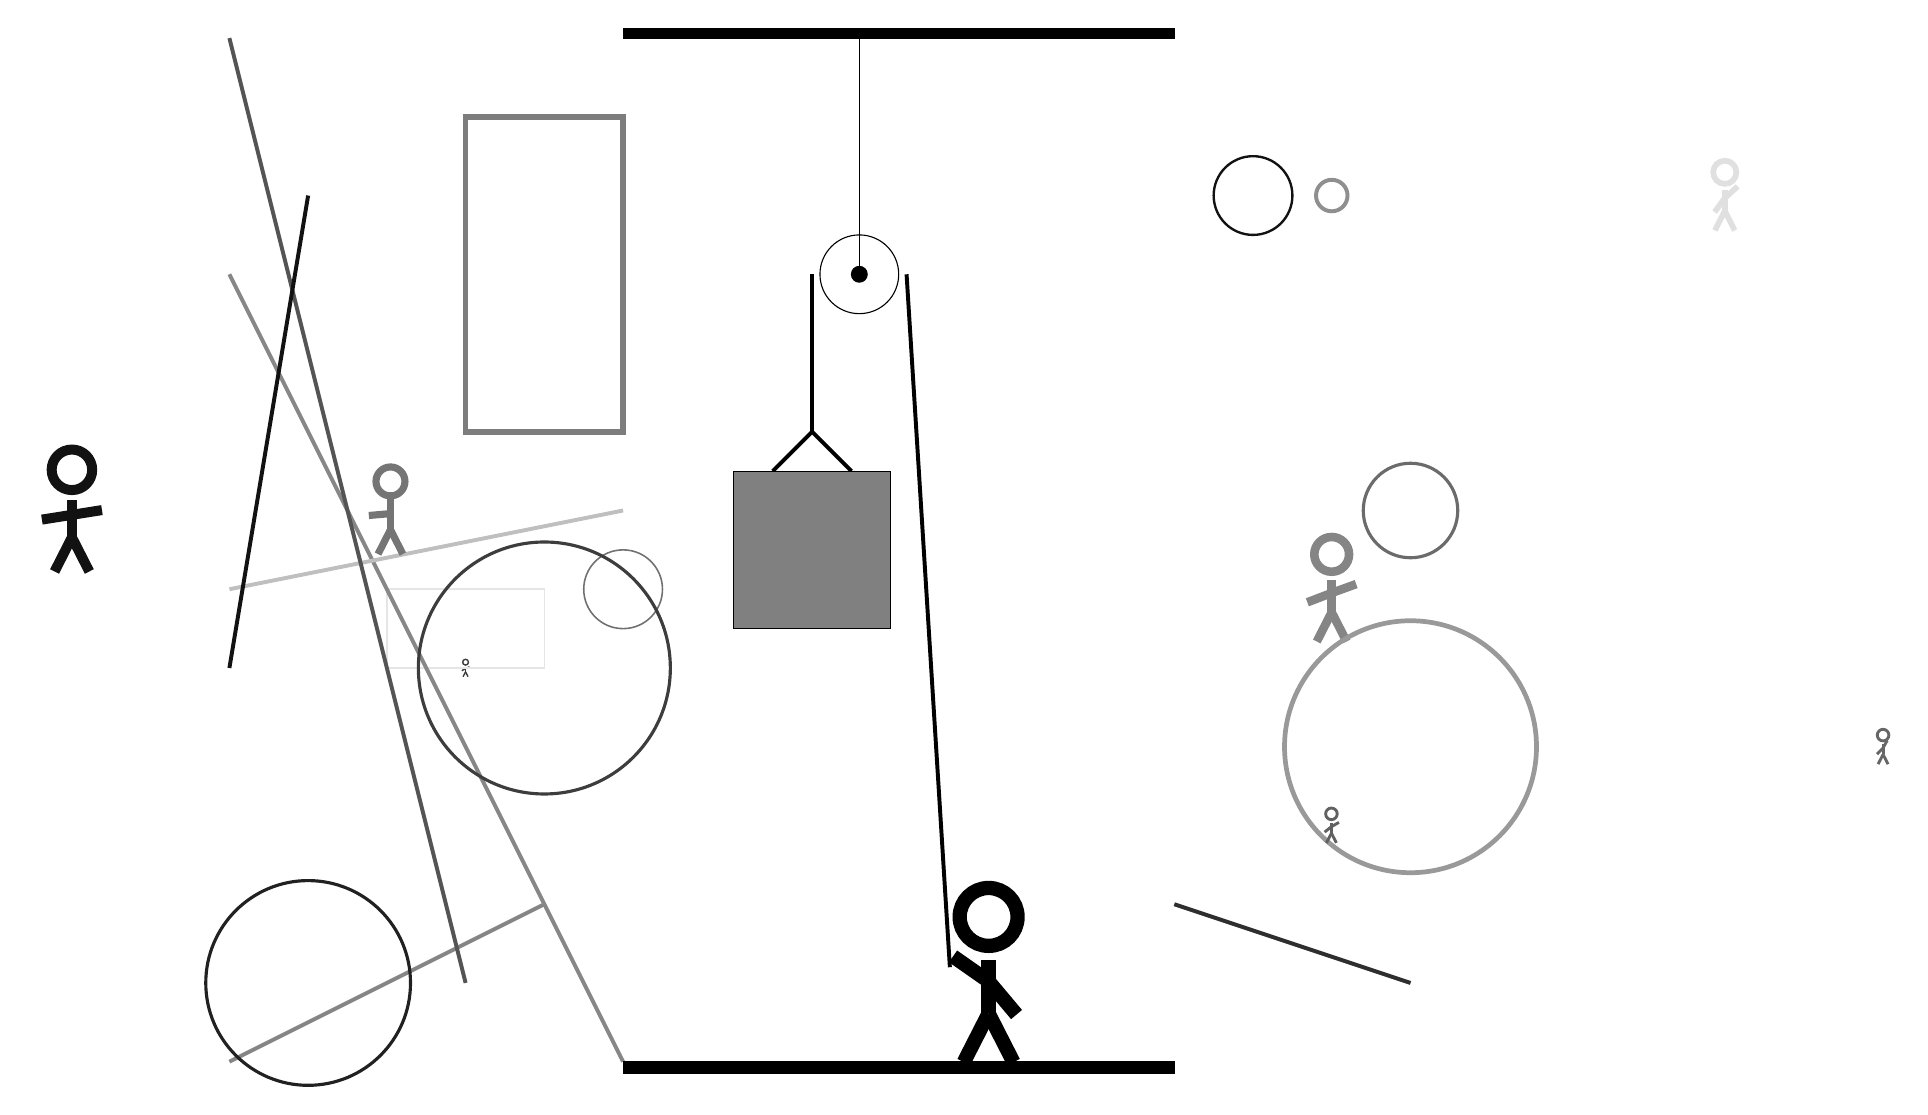
\begin{tikzpicture}
		%%%%% START %%%%%
		
		\draw[fill=black] (-2, 10) rectangle (5, 10.125);
		
		\draw (1, 7) circle (0.5);
		\draw[fill=black] (1, 7) circle (0.1);
		\draw (1, 10) -- (1, 7);
		
		\draw[line width=0.5mm] (-0.1, 4.5) -- (0.4, 5.0) -- (0.9, 4.5);
		\draw[fill=black!50] (-0.6, 4.5) rectangle (1.4, 2.5);
		
		\node[line width=0.7mm, color=black!93] at (-9, 4) {\Strichmaxerl[7][9][9]};
		
		\node[line width=0.5mm, color=black!48] at (7, 3) {\Strichmaxerl[6][21][20]};
		\draw[line width=0.7mm, color=black!51] (-2, 9) rectangle (-4, 5);
		\draw[line width=0.5mm, color=black!82](5, -1) -- (8, -2);
		\draw [line width=0.4mm, color=black!61](10, -1) circle (0.0);
		
		\draw[line width=0.5mm, color=black!48](-3, -1) -- (-7, -3);
		\draw [line width=0.2mm, color=black!56](-2, 3) circle (0.5);
		
		\node[line width=0.5mm, color=black!76] at (-4, 2) {\Strichmaxerl[1][29][25]};
		\draw[line width=0.2mm, color=black!10] (-3, 2) rectangle (-5, 3);
		\draw[line width=0.5mm, color=black!47](-7, 7) -- (-2, -3);
		\node[line width=0.6mm, color=black!60] at (14, 1) {\Strichmaxerl[2][46][61]};
		\draw[line width=0.5mm, color=black!25](-2, 4) -- (-7, 3);
		\draw [line width=0.4mm, color=black!76](-3, 2) circle (1.6);
		\draw [line width=0.6mm, color=black!40](8, 1) circle (1.6);
		\draw[line width=0.5mm, color=black!67](-7, 10) -- (-4, -2);
		\draw [line width=0.4mm, color=black!87](-6, -2) circle (1.3);
		\draw[line width=0.5mm, color=black!93](-6, 8) -- (-7, 2);
		\node[line width=0.3mm, color=black!12] at (12, 8) {\Strichmaxerl[4][54][42]};
		\node[line width=0.3mm, color=black!62] at (7, 0) {\Strichmaxerl[2][38][30]};
		
		\draw [line width=0.4mm, color=black!58](8, 4) circle (0.6);
		\draw [line width=0.3mm, color=black!93](6, 8) circle (0.5);
		
		\draw [line width=0.5mm, color=black!44](7, 8) circle (0.2);
		\node[line width=0.7mm, color=black!54] at (-5, 4) {\Strichmaxerl[5][5][90]};
		
		\draw[line width=0.5mm] (0.4, 7) -- (0.4, 5.0);
		\centerarc[line width=0.5mm](1, 7)(0:180:0.6);
		\draw[line width=0.5mm](1.6, 7) -- (2.15, -1.8);
		
		\node at (2.6, -1.9) {\Strichmaxerl[10][-35][-50]};
		
		\draw[fill=black] (-2, -3) rectangle (5, -3.15);
		
		%%%%% END %%%%%
	\end{tikzpicture}
\end{document}